\section{Question 2}\label{sec:q2}    
\subsection{2a}
\textit{To facilitate a precision landing in an otherwise safe environment
the addition of multiple advanced systems to the standard GNC system is necessary. Describe (in detail) at least three systems that are either completely new or need con-siderable changes with respect to the standard GNC system.}\\

The three systems are Terrain Absolute Navigation (TAN), Terrain Relative Navigation (TRN) and Hazard Detection and Avoidance (HDA).\\

A vehicle equipped with \textbf{Terrain Absolute Navigation} has a pre-determined map of the surface of the body on board. For example, if this body is the moon, the vehicle has a map of the lunar surface. TAN then uses sensors that can detect features on the surface, and then compare these with the on-board map to determine the location. Sensors may be optical, but radar or LIDAR sensors can also be used. The inputs for TAN are therefore the data from the surface sensors and the data from the on-board map as inputs, and can produce altitude, position, relative speed, and heading as outputs.\\

Alternatively, if no detailed map of the surface is available, \textbf{Terrain Relative Navigation} can be used. This method uses similar sensors to look at the surface below, and take a image. However, it then compares this image to the previously taken image. By using algorithms that can detect features of the landscape, it can determine speeds and headings relative to the surface. This can also be seen in the figure.
\begin{figure}[H]
    \centering
    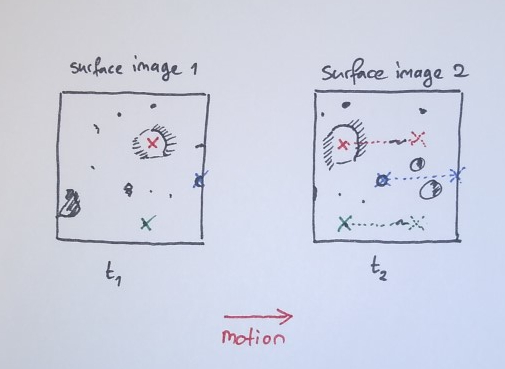
\includegraphics[width=0.5\columnwidth]{Figures/picture_TRN.jpg}
    \caption{The principle behind TRN}
    \label{fig:TRN}
\end{figure}

Lastly, \textbf{Hazard Detection and Avoidance} is a more advanced system to ensure a safe landing and provide the lander with a higher level of autonomy. This system includes sensory equipment that can accurately provide a 3D map of the prospected landing area. Usually LIDAR is used, but radio doppler sensors work also. Using computer algorithms, potential hazards can be identified, and poor landing zones can be rejected in favour of better suited ones. The outputs of the system can therefore be, besides velocity and relative position, coordinates for better landing locations.

\subsection{2b}
\textit{Draw the standard GNC flowchart and add the systems described in (a) to
the chart. Clearly indicate which blocks are from the standard system and which are only needed for a precision landing.}\\
See lecture notes section 9-9.
\begin{figure}[H]
    \centering
    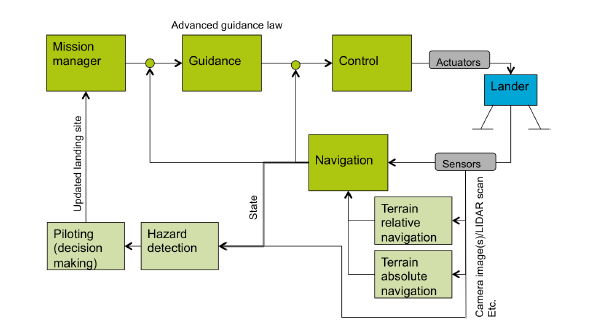
\includegraphics[width=0.8\columnwidth]{Figures/GNCplus.PNG}
    \caption{A GNC system with TAN, TRN, and HDA}
    \label{fig:GNC}
\end{figure}


\subsection{2c}
The topic of E-guidance is no longer part of the study material for this course, and is therefore omitted from this guide.